\chapter{Model Inference and Revision}
\begin{mybox}
In the previous chapter, we introduced several approaches of refined reachability analysis, which are more suitable for practical use (more efficient and more conclusive).
Nevertheless, these approaches can never take effect no matter how powerful they are, if the original model does not reflect the reality.

To model a biological computational system, one may consider two possible aspects: a first-step model built by biologists (variables, some confirmed transitions, some \textit{a priori} properties etc.) and the observation of the experiments (time-series data, steady states, oscillations, etc.).

This chapter is dedicated to the introduction of three different approaches of model inference/revision:

\begin{itemize}
    \item \textit{via} reachability properties and candidate regulations
    \item \textit{via} partial correlation (statistics)
    \item \textit{via} reachability properties and time-series data
\end{itemize}

There lies very little nuance between model inference and model revision: these two operations begin with some \textit{a priori} information and/or observations, aiming at constructing a new model/modifying an existed model.
As a result, they take the information apart from the existing transitions into account, using different tools to transform this information into possible transitions in the model (also can modify or deny existing transitions).

\end{mybox}

\section{Background}
Model inference/learning can be useful not only in biology \cite{ribeiro2015learning} but also in other domains with the need of abstraction, e.g. robotics \cite{nguyen2011model}, multi-agent systems \cite{foerster2016learning}.
In the community of bioinformatics, DREAM  challenge\footnote{\url{http://dreamchallenges.org/about-dream}} is a well-known organization calling for the participation of the whole world on the newest bio-medical problems (called challenges). 
Among these challenges, some of them are in the domain of inference and prediction:
DREAM2\footnote{\url{https://www.synapse.org/\#!Synapse:syn2825374/wiki/71143}},
DREAM4\footnote{\url{https://www.synapse.org/\#!Synapse:syn2825304/wiki/71129}},
DREAM8\footnote{\url{https://www.synapse.org/\#!Synapse:syn1720047/wiki/55342}},
DREAM11\footnote{\url{https://www.synapse.org/\#!Synapse:syn6131484/wiki/402026}}.

Like in biology, the modeling structures in robotics are usually complex and with big size, which is difficult in control, prediction and simulation.
Constructing an abstracted (often approximated) model is a compromising way of dealing with the complexity.
However, the abstracted models are theoretically non-equivalent with the original ones because they contain different amount of information.
As long as the equivalence is impossible, we wish that the abstracted models are in bisimulation with the original ones with respect to certain variables and keep certain important properties.

Concretely speaking, we developed three approaches which are to be presented in this chapter:

\begin{enumerate}
    \item Constructing models from incomplete model and candidate regulations plus dynamic constraints
    \item Inferring models from continuous observation data
    \item Least revising existing models via \textit{a priori} knowledge (mainly reachability information)
\end{enumerate}

Among the three approaches, intuitively approach 1 has the least complexity. 
Because the most naive method, \textit{i.e.} brute force search is to verify every combination of the candidates if it satisfies the constraints. 
The models to be verified are of $O(2^n)$, where $n$ is the number of candidate transitions.
For approach 2, to explain a transition $A\to a_i$, there are at most $m-1$ possibilities for $A$ has one local state, $C_{m-1}^2$ possibilities for $A$ has 2 local states \ldots where $m$ is the number of variables.
Similarly, approach 3 also has a factorial complexity.

\section{Model Inference \textit{via} Candidate Regulations}
We begin with the problem which seems to have the smallest complexity.
The completely exhaustive solution that we just presented is still meaningless in real application.
Roughly speaking, we aim at finding the transitions among the candidates which meet the unsatisfied constraints and keep satisfied constraints satisfied.

\subsection{Problem Description}
Briefly speaking, completion problem is: incomplete model + candidate regulations + constraints $\to$ complete model.
The complete model contains all the elements in the incomplete model and consistent with all the \textit{a priori} information. 

\begin{definition}[Model completion]
    Given an incomplete ABAN $AB=(\Sigma, L, T)$ (where $T$ can be empty), a complete model is an ABAN $AB'=(\Sigma, L, T')$ which satisfies $T'\supseteq T$, $AB'$ consistent with the set of reachability constraints $C$ and the completion set $CS=T'\setminus T$ is consistent with the set of candidate regulations $R$, where
    \begin{itemize}
        \item $R=\{(body,head,sgn)\mid body\in \Sigma,\ head\in \Sigma,\ sgn\in \{0,1\}\}$ 
        \item $C=\{(\alpha,\omega,r)\mid\alpha \in L,\ \omega\in LS,\ r\in \{\mathbf{True,False}\}\}$
    \end{itemize}
\end{definition}

$R$ shows the possible relations between variables, $body$ may inhibit (0) or promote (1) $head$.
$C$ shows the \textit{a priori} reachability, $\omega$ is (un)reachable from $\alpha$.
The definition of consistency is straightforward, but is different for reachability constraints and candidate regulations.

\begin{definition}[Consistency]
\leavevmode
\makeatletter
\@nobreaktrue
\makeatother
\begin{itemize}
    \item An ABAN $AB$ is said consistent with a with the set of reachability constraints $C$ iff $\forall (\alpha,\omega,r)\in C$ s.t. $reach(\alpha,\omega)=r$
    \item A completion set $CS$ is said consistent with a with the set of candidate regulations $R$ if $\forall \acm{a_i}{b_{1-j}}{b_j}\in CS, \exists (body,head,sgn)\in R$ s.t. $body=a,\ head=b,\ (i=j)=sgn$. 
\end{itemize}
    
\end{definition}
Theoretically, to obtain a good new ABAN, we have to assure $T$ has no \textit{bad} transitions, because the completion operation is not able to remove bad transitions. 

Before our research began, Paulev\'e \textit{et al.} had worked on cut-sets for reachability in large scale automata networks \cite{PAK13-CAV}, which is the reverse operation of completion set.
It can eliminate certain transitions according to unreachability properties.
By combining these two operations, one can construct/revise a model according to \textit{a priori} information (candidate regulations) and constraints (reachability).

As stated in the previous chapter, exact reachability is a hard task.
We use two criteria, over-approximation and under-approximation to replace the notion of reachability (shown in Figure \ref{fig:vennDiagram}).

%In the context of SLCG, completion is defined as follows: given a state sequence $S$ of observation and a set of possible regulations $H$ (in the form of ABAN) to be verified, find the minimum subset of $H$ such that $S$ is realizable from initial state.

\subsection{Completion by Over-Approximation}
Over-approximation is the reasoning of pseudo-reachability in Definition \ref{defPseudoReach}. 
It associates local states and transitions with the initial state according to the causalities: if there exists a pathway from the target local state to the initial state, this target state can be reachable.
Over-approximation does not take into consideration the order of transitions to be fired, which is the cause of inconclusiveness (literally it over-approximates the reachability).
Thus over-approximation is a necessary condition.

Figure \ref{CompOv} gives a first intuition of the idea.
The visualization of the set of candidate regulations $R=\{(a,b,+),(c,a,-)\}$ is on the left.
On the right, the initial ABAN has only three variables $\Sigma=\{a,b,c\}$ and initial state $\langle a_0,b_0,c_0\rangle$, with $T=\{\acm{a_1}{b_0}{b_1}\}$.
$b_1$ is not reachable because of the unreachability of $a_1$.
As $(c,a,-)\in R$, \ac{c_0}{a_0}{a_1} is added then $a_1$ becomes reachable which makes $b_1$ also reachable.
$T'=\{\acm{a_1}{b_0}{b_1},\acm{c_0}{a_0}{a_1}\}$, $CS=\{\acm{c_0}{a_0}{a_1}\}$.

\begin{figure}[ht]
\centering
\begin{minipage}{0.5\linewidth}
\centering
\begin{tikzpicture}
\coordinate (P1) at (0,0);
\node at (P1) {{\Large c}};
\coordinate (P2) at (2,0);
\node at (P2) {{\Large a}};
\coordinate (P3) at (4,0);
\node at (P3) {{\Large b}};
\coordinate (P4) at ($(P2)+(150:0.6)$);
\draw (P1) circle(0.4) ;
\draw (P2) circle(0.4);
\draw (P3) circle(0.4);
\draw [line width=1pt](30:0.5) .. controls  (1,0.7) .. (P4);
\draw [->, line width=1pt]($(P2)+(30:0.5)$) .. controls  (3,0.7) .. ($(P3)+(150:0.55)$);
\draw [line width=1pt]($(P4)+(45:0.15)$) -- ($(P4)-(45:0.15)$);
\end{tikzpicture}
\end{minipage}
\hfill
\begin{minipage}{0.5\linewidth}
\centering
\begin{tikzpicture}
\TSort{(0,0)}{c}{2}{l}
\TSort{(2,0)}{a}{2}{r}
\TSort{(4,0)}{b}{2}{r}
\THit{a_1}{}{b_0}{.west}{b_1}
\THit{c_0}{dashed,thick,color=red}{a_0}{.west}{a_1}


\path[bounce,bend left]
\TBounce{b_0}{}{b_1}{.west}
\TBounce{a_0}{thick,color=red}{a_1}{.west}
;
\TState{a_0,b_0,c_0}
\end{tikzpicture}
\end{minipage}

\caption[Completion by over-approximation]{Completion by over-approximation. Dashed arrows represent added action.}\label{CompOv}
\end{figure}
Algorithm \ref{algComOver} shows the detailed algorithm.

\subsection{Completion by Under-Approximation}
Over-approximation is only a necessary condition of reachability.
If one wants to guarantee the reachability even in the price of redundant transitions, he may consider the completion by under-approximation.

Under-approximation is another reasoning of LCG. 
It associates \textit{all} the local states with the initial state which may appear instead of the initial state.
This association covers all the orders of occurrence.
Likewise, in the LCG, if there is a pathway from certain local state and the initial state, this state \textit{should} be reachable.

However, all the orders of occurrence do not necessarily appear during the simulation, which suggest that this approach ``under-approximates'' the reachability.

Additionally, the computation of under-approximation is more complicated than over approximation, as the set of associated local states grows during the computation.
Former added local states need to be regarded as new ``target states''.
This process is called \textit{update}. 
Update does not stop until the set of associated local states becomes stable.

\begin{definition}[Under-approximation]
    
\end{definition}

Let us take the Asynchrhonous Automata Network $AAN=(\Sigma, L, T)$ in Figure \ref{ExUnder} as example with $\Sigma= \{a,b,c,d\}$, $T=\{\acm{b_1}{a_0}{a_1}, \acm{b_1}{d_0}{d_1},\acm{c_1}{a_1}{a_2}, \acm{d_0}{b_0}{b_1}\}$, initial state $\langle a_0,b_0,c_0,d_0\rangle$.
With candidate regulations $R=\{(d,c,-),(c,d,-)\}$, Figure \ref{Under1}, Figure \ref{Under2} and Figure \ref{Under3} show the procedures of under-approximation: after two additions of actions and an update, the LCG becomes stable and $a_2$ is reachable.
$T'=\{\acm{b_1}{a_0}{a_1}, \acm{b_1}{d_0}{d_1},\acm{c_1}{a_1}{a_2}, \acm{d_0}{b_0}{b_1},\acm{d_1}{c_0}{c_1}, \acm{c_1}{d_1}{d_0}\}$, $CS=\{\acm{d_1}{c_0}{c_1}, \acm{c_1}{d_1}{d_0}\}$.

\begin{figure}[ht]
\centering
%\begin{tikzpicture}
%\TSort{(3,0)}{a}{3}{l}
%\TSort{(0,0)}{b}{2}{l}
%\TSort{(6,0)}{c}{2}{r}
%\TSort{(2,-2)}{d}{2}{b}
%\THit{b_1}{}{a_0}{.north west}{a_1}
%\THit{c_1}{}{a_1}{.east}{a_2}
%\THit{d_0}{distance=90,out=240,in=210}{b_0}{.west}{b_1}
%\THit{b_1}{}{d_0}{.north}{d_1}
%\THit{d_0}{distance=90,out=-75,in=-45,dashed,thick,color=red}{c_0}{.east}{c_1}
%\THit{c_1}{dashed,thick,color=red}{d_1}{.north}{d_0}
%
%
%\path[bounce,bend right]	
%\TBounce{a_1}{}{a_2}{.east}
%\TBounce{d_1}{thick,color=red}{d_0}{.north east}
%\TBounce{c_0}{thick,color=red}{c_1}{.east}
%;
%\path[bounce,bend left]
%\TBounce{a_0}{}{a_1}{.west}
%\TBounce{b_0}{}{b_1}{.west}
%\TBounce{d_0}{}{d_1}{.north west}
%;
%\TState{a_0,b_0,c_0,d_0}
%\end{tikzpicture}
\begin{tikzpicture}[apdotsimple/.style={apdot}]
\scriptsize
\TSort{(0,0)}{a}{2}{l}
\TSort{(2,0)}{b}{2}{l}
\TSort{(4,0)}{c}{2}{l}
\TSort{(6,0)}{d}{2}{l}

% with delays
\path[local transitions]

	(a_0) edge node[auto] {\{$b_1, c_1$\}} (a_1)
	
	(b_0) edge node[auto] {$\{d_0\}$} (b_1)
	(d_0) edge node[auto] {$\{b_1\}$} (d_1)
	(d_1) edge[dashed,color=red] node[auto] {$\{c_1\}$} (d_0)
	%(c_1) edge node[auto] {$\{b_0\}$, $2$} (c_0)
	(c_0) edge[dashed,color=red] node[auto] {$\{d_1\}$} (c_1)
;

\TState{a_0, b_0, c_0, d_0}


\end{tikzpicture}

\caption[Completion by under-approximation]{Example of completion by under-approximation. Dashed arrows represent added actions.}\label{ExUnder}
\end{figure}

In Figure \ref{Under1}, \fbox{$c_1$} unreachable then the joint state $\langle b_1, c_1\rangle$ is not reachable, $a_2$ is not reachable .

\begin{figure}[ht]
\centering
\begin{tikzpicture}
\node (O1) at (0,0) {$a_0\Rsh^*a_2$};
\node[draw] (Pm1) at (-1.75,0) {$a_2$};
\draw[->] (Pm1)-- (O1);
\node (S1) at ($(O1)+(1.5,0)$){};
\draw[->] (O1) -- (S1);
\draw (S1) circle (3pt);
\node[draw] (P1) at ($(S1)+(1,1)$){$b_1$};
\node[draw] (P2) at ($(S1)+(1,-1)$){$c_1$};
\draw[->] (S1)--(P1);
\draw[->] (S1)--(P2);
\node (O2) at ($(P1)+(1.75,0)$) {$b_0\Rsh^*b_1$};
\node (O3) at ($(P2)+(1.75,0)$) {$\perp$};
\draw[->] (P1)--(O2);
\draw[->] (P2)--(O3);
\node (S2) at ($(O2)+(1.5,0)$){};
\draw (S2) circle (3pt);
\draw[->] (O2) -- (S2);
\node[draw] (P3) at ($(S2)+(1,0)$){$d_0$};
\draw[->] (S2) -- (P3);
\node (O5) at ($(P3)+(1.75,0)$) {$d_0\Rsh^*d_0$};
\draw[->] (P3)--(O5);
\node (S5) at ($(O5)+(1.5,0)$){};
\draw (S5) circle (3pt);
\draw[->] (O5) -- (S5);
\end{tikzpicture}
\caption[Operations on LCG(1)]{Step 1, under-approximation LCG of Figure \ref{ExUnder} studying the reachability of $a_2$ (small circles stand for solutions and squares stand for processes). }\label{Under1}
\end{figure}

In Figure \ref{Under2}, according to candidate regulation ${(d,c,-)}\in R$, \ac{d_1}{c_0}{c_1} is added, but the reachability of under-approximation requires all the possible occurrences are realizable, e.g. transition $d_1\Rsh^*d_0$ must be firable.

\begin{figure}[ht]
\centering
\begin{tikzpicture}
\node (O1) at (0,0) {$a_0\Rsh^*a_1$};
\node[draw] (Pm1) at (-1.75,0) {$a_1$};
\draw[->] (Pm1)-- (O1);
\node (S1) at ($(O1)+(1.5,0)$){};
\draw[->] (O1) -- (S1);
\draw (S1) circle (3pt);
\node[draw] (P1) at ($(S1)+(1,1)$){$b_1$};
\node[draw] (P2) at ($(S1)+(1,-1)$){$c_1$};
\draw[->] (S1)--(P1);
\draw[->] (S1)--(P2);
\node (O2) at ($(P1)+(1.75,0)$) {$b_0\Rsh^*b_1$};
\node (O3) at ($(P2)+(1.75,0)$) {$c_0\Rsh^*c_1$};
\draw[->] (P1)--(O2);
\draw[->] (P2)--(O3);
\node (S2) at ($(O2)+(1.5,0)$){};
\draw (S2) circle (3pt);
\draw[->] (O2) -- (S2);
\node (S3) at ($(O3)+(1.5,0)$){};
\draw[fill=black] (S3) circle (3pt);
\draw[->] (O3) -- (S3);
\node[draw] (P3) at ($(S2)+(1,0)$){$d_0$};
\draw[->] (S2) -- (P3);
\node[draw] (P4) at ($(S3)+(1,0)$){$d_1$};
\draw[->] (S3) -- (P4);
\node (O4) at ($(P3)+(30:1.75)$) {$d_0\Rsh^*d_0$};
\node (O5) at ($(P3)+(1.75,0)$) {$d_1\Rsh^*d_0$};
\draw[->] (P3)--(O4);
\draw[->] (P3)--(O5);
\node (O6) at ($(P4)+(-30:1.75)$) {$d_1\Rsh^*d_1$};
\node (O7) at ($(P4)+(1.75,0)$) {$d_0\Rsh^*d_1$};
\draw[->] (P4)--(O6);
\draw[->] (P4)--(O7);
\node (S4) at ($(O4)+(1.5,0)$){};
\draw (S4) circle (3pt);
\draw[->] (O4) -- (S4);
\node (S5) at ($(O5)+(1.5,0)$){$\perp$};
\draw[->] (O5) -- (S5);
\node (S6) at ($(O6)+(1.5,0)$){};
\draw[fill=black] (S6) circle (3pt);
\draw[->] (O6) -- (S6);
\node (S7) at ($(O7)+(1.5,0)$){};
\draw[fill=black] (S7) circle (3pt);
\draw[->] (O7) -- (S7);
\draw[->] ($(S7)+(0,3pt)$) -- (P1);
\end{tikzpicture}
\caption[Operations on LCG(2)]{Step 2 of completion by under-approximation (filled small circles stand for new possible solutions after completion).}\label{Under2}
\end{figure}

In Figure \ref{Under3}, the completed under-approximation LCG shows $a_2$ is now reachable after adding $\acm{c_1}{d_1}{d_0}$ according to ${(c,d,-)}\in R$.

\begin{figure}[ht]
\centering
\begin{tikzpicture}[>=stealth]
\node (O1) at (0,0) {$a_0\Rsh^*a_1$};
\node[draw] (Pm1) at (-1.75,0) {$a_1$};
\draw[->] (Pm1)-- (O1);
\node (S1) at ($(O1)+(1.5,0)$){};
\draw[->] (O1) -- (S1);
\draw (S1) circle (3pt);
\node[draw] (P1) at ($(S1)+(1,1)$){$b_1$};
\node[draw] (P2) at ($(S1)+(1,-1)$){$c_1$};
\draw[->] (S1)--(P1);
\draw[->] (S1)--(P2);
\node (O2) at ($(P1)+(1.75,0)$) {$b_0\Rsh^*b_1$};
\node (O3) at ($(P2)+(1.75,0)$) {$c_0\Rsh^*c_1$};
\draw[->] (P1)--(O2);
\draw[->] (P2)--(O3);
\node (S2) at ($(O2)+(1.5,0)$){};
\draw (S2) circle (3pt);
\draw[->] (O2) -- (S2);
\node (S3) at ($(O3)+(1.5,0)$){};
\draw (S3) circle (3pt);
\draw[->] (O3) -- (S3);
\node[draw] (P3) at ($(S2)+(1,0)$){$d_0$};
\draw[->] (S2) -- (P3);
\node[draw] (P4) at ($(S3)+(1,0)$){$d_1$};
\draw[->] (S3) -- (P4);
\node (O4) at ($(P3)+(30:1.75)$) {$d_0\Rsh^*d_0$};
\node (O5) at ($(P3)+(1.75,0)$) {$d_1\Rsh^*d_0$};
\draw[->] (P3)--(O4);
\draw[->] (P3)--(O5);
\node (O6) at ($(P4)+(-30:1.75)$) {$d_1\Rsh^*d_1$};
\node (O7) at ($(P4)+(1.75,0)$) {$d_0\Rsh^*d_1$};
\draw[->] (P4)--(O6);
\draw[->] (P4)--(O7);
\node (S4) at ($(O4)+(1.5,0)$){};
\draw (S4) circle (3pt);
\draw[->] (O4) -- (S4);
\node (S5) at ($(O5)+(1.5,0)$){};
\draw[fill=black] (S5) circle (3pt);
\draw[->] (O5) -- (S5);
\node (S6) at ($(O6)+(1.5,0)$){};
\draw (S6) circle (3pt);
\draw[->] (O6) -- (S6);
\node (S7) at ($(O7)+(1.5,0)$){};
\draw (S7) circle (3pt);
\draw[->] (O7) -- (S7);
\draw[->] ($(S5)-(0,3pt)$) -- (P2);
\draw[->] ($(S7)+(0,3pt)$) -- (P1);
\end{tikzpicture}
\caption[Operations on LCG(3)]{Step 3 of completion by under-approximation (filled small circles stand for new possible solutions after completion).}\label{Under3}
\end{figure}

Algorithm \ref{algComUnder} shows the whole process.

Also, if one wants to study the candidate transitions with multiple variables in the head, he can also replace regulations with transitions, using the same process to complete the ABAN. 

\section{Model Inference via Statistics}

In the previous contents, only the systems with delay 1 are discussed (BN, ABAN, etc.), i.e. the influence done by variables will take place at the next time point (immediately).
However, in biological context, some reactions have a long duration, and some even need a whole observation period to take place.
For this reason, we require approaches to reveal transitions of different delays: for an observation of period $T$, possible delays lie in $[1,T-1]$.

\subsection{Preliminaries}
In Section \ref{sec:regNetwork}, the definition of regulatory network requires every regulation take effect immediately, as the definition is originally related to ordinary differential equations \cite{khalis2009smbionet}.

To integrate the notion of delay into regulatory network, we modify the definition of regulatory network.
\begin{definition}[Regulatory network with delay]
A biological regulatory graph is a labeled directed graph $G=(V,E)$ where 
\begin{itemize}
    \item each vertex $v$ of $V$, called variable, is provided with a boundary $b_v\in \mathbb{N}$ less or equal to the out-degree of v in G.
    \item each arc $u\in v$ of $E$ is labelled with a couple ($t_{uv}$, $\alpha_{uv}$) where $t_{uv}$ is an integer between 1 and $b_v$, called qualitative threshold and where $\alpha_{uv}\in \{+,-\}$ is the sign of the regulation.
\end{itemize}
\end{definition}


With the new formalization, we can describe the inference problem in a broader way.



\subsection{Partial Correlation}
Spearman: Pearson on ranking

In huge biological networks, it is not possible to calculate hypotheses by hand nor to traverse all the possible addable transitions, as stated formerly, the verification of $\mathcal{O}(3^{|Global States|})$ states is a huge task (for any component, each of other components has 3 possibilities, promotion, inhibition and no regulation).
 
To deal with the great complexity of verification, \textit{a priori} knowledge is needed. 
Some unsatisfied states can be eliminated without global verification.  
In order to take all the information into account, statistical approaches come into sight.
They try to find relations between different components from the observation of all the time points.

One additional profit of statistical approaches is that original time series data are discretized before being used, which cause a loss of information.
This loss could lead to an imprecise model.
However, some statistical approaches could use directly the continuous time series data as input which avoid this difficulty.

\subsubsection{Overall Process}
We proposed a method applying partial correlation to detect the relevance of each pair of components.

\begin{figure}[ht]
\begin{tikzpicture}[node distance = 1.5cm, auto]
    % Place nodes
    \node [block] (originalData) {Time-series data};
    \node [block, right = of originalData] (dataDiscretization) {Data discretization};
     \node [block, right = of dataDiscretization] (varReconstruction) {Variable reconstruction};
    \node [block, below = of originalData] (ranking) {Sorting};
    \node [block, right = of ranking] (changeRate) {Change rate};
    \node [block, below = of ranking] (dataReg) {Data regrouping \& Spearman coefficient};
     \node [block, right = of dataReg] (partialCoeff) {Partial coefficient};
     \node [block, right = of partialCoeff] (regulations) {Regulations $x\xrightarrow{+/-}y$};
     \node [block, below = of varReconstruction] (actions) {Transitions \ac{x_i}{y_j}{y_k}};
     \coordinate [left = of ranking,node distance=0.5cm](abstract);
    % Draw edges
    \path [line] (originalData) -- (dataDiscretization);
    \path [line] (originalData) -- (ranking);
    \path [line] (originalData) -- (changeRate);
    \path [line] (changeRate) -- (ranking);
    \path [line,dashed] (dataDiscretization) -- (varReconstruction);
    \path [line] (varReconstruction) -- (ranking);
    \path [line] (ranking) -- (dataReg);
    \path [line] (dataReg) -- (partialCoeff);
    \path [line] (partialCoeff) -- (regulations);
    \path [line,dashed] (regulations) -- (actions);
    \path [line,dashed] (originalData) -|  (abstract)node[rotate=90,below=2pt]{Pearson Coefficient} |-(dataReg);
\end{tikzpicture}
\caption[Workflow of model inference via partial correlation]{Workflow of the whole procedure of hypotheses generation (dashed arrows stand for optional processes)}\label{plan}
\end{figure}
Figure \ref{plan} shows the procedure of regulation generation: before discretizing original data, Pearson or Spearman correlation coefficient \cite{samaga2009logic,hauke2011comparison} are calculated for identifying the relevance between original data and change rates of components (in linear or monotonic way respectively). If cooperation between components exists, former coefficients need replacing by partial ones \cite{de2004discovery} for more precise result.
Resulting coefficients above the threshold (One can set a threshold of relevance, e.g. 0.7) suggest there probably exist regulations between components.

Furthermore, to complete Biological Regulatory Networks in form of Automata Network, more accurate regulations are inferred through variable reconstruction, which splits a variable into several new variable according to its qualitative levels.
For example, component $a$ has two discrete levels $a_0$ $a_1$, then correlation coefficients as well as partial coefficients are calculated in the domain of $a_0$ and of $a_1$ separately.
As a result, the relevance between $a_0$ and other components and that of $a_1$ are calculated, with which possible addable actions of ABAN are deduced.

As all the subroutines depicted in Figure \ref{plan} are implemented, starting from original data, regulations in form of Thomas' model or ABAN are resulted step by step. In the next, the data treatments Figure \ref{plan} will be introduced with examples.

%\subsection{Partial Correlation Coefficients}
\subsection{Data Regrouping}
To gain a better understanding of correlations between observation data and change rate, certain observed data of one component are replaced by corresponding change rate. By calculating the correlation coefficients of such matrix, regulation on this component is characterized.

Example:

$$\kbordermatrix{\mbox{}&t_0&t_1&t_2&t_3\\
a&a_{t_0}&a_{t_1}&a_{t_2}&a_{t_3}\\
b&b_{t_0}&b_{t_1}&b_{t_2}&b_{t_3}\\
c&c_{t_0}&c_{t_1}&c_{t_2}&c_{t_3}\\
d&d_{t_0}&d_{t_1}&d_{t_2}&d_{t_3}
}
\to\kbordermatrix{\mbox{}&t_0&t_1&t_2\\
a'&a'_{t_0}&a'_{t_1}&a'_{t_2}\\
b&b_{t_0}&b_{t_1}&b_{t_2}\\
c&c_{t_0}&c_{t_1}&c_{t_2}\\
d&d_{t_0}&d_{t_1}&d_{t_2}
}$$

With delay = 1 time unit, $a'$ is the change rate of $a$, calculated via 
$$a'=\dfrac{\mathrm{d}a(t)}{\mathrm{d}t}=\dfrac{a(t+1)-a(t)}{(t+1)-t}=a(t+1)-a(t)$$ In this way, regulations of $b,c,d$ on $a$ are then evaluated by aforementioned coefficients. Also matrices representing different delays can be formed analogously.

\subsection{Inference of Different Delay using Variable Reconstruction}
By applying aforementioned approaches, regulations in the form of $a\xrightarrow{+/-}b$ are deduced, but the result is not in the precise form of ABAN. To obtain a result in such form, variable reconstruction is compulsory.

\begin{figure}[ht]
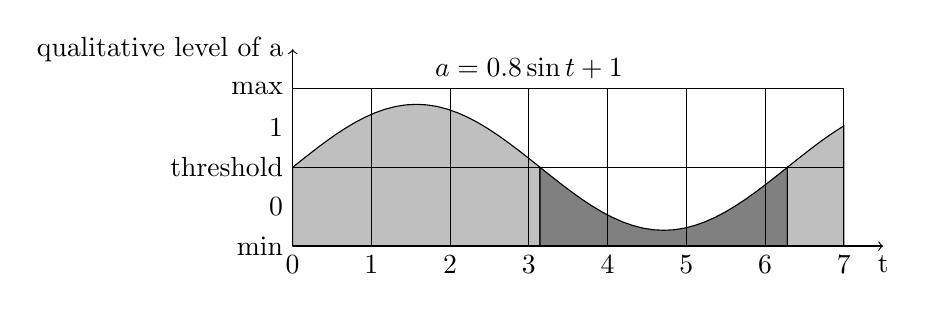
\begin{tikzpicture}
\draw[->] (0,0) -- (0,2.5);
\draw[->] (0,0) -- (7.5,0);
\draw(0,2)node[left]{max};
\draw(0,0)node[left]{min};
\draw(0,1)node[left]{threshold};
\foreach \y in {0,1} \draw(0,\y+0.5)node[left]{\y};
\foreach \x in {0,1,...,7} \draw(\x,0)node[below]{\x};
\filldraw[draw=black,fill=black!25!white]
	plot[domain=0:pi] (\x, {0.8*sin(\x r)+1})--(pi,0)--(0,0)--(0,1); 
\filldraw[draw=black,fill=gray]
	plot[domain=pi:2*pi] (\x, {0.8*sin(\x r)+1})--(2*pi,0)--(pi,0)--(pi,1); 
\filldraw[draw=black,fill=black!25!white]
	plot[domain=2*pi:7] (\x, {0.8*sin(\x r)+1})--(7,0)--(2*pi,0)--(2*pi,1); 
\draw[step=1] (0,0) grid (7,2);
\draw (7.5,0) node[below]{t};
\draw (0,2.5) node[left]{qualitative level of a};
\draw(3,2)node[above]{$a=0.8\sin t+1$};
\end{tikzpicture}
\caption[Variable reconstruction]{Example of variable reconstruction, former variable $a=0.8\sin t+1(t\in [0,7])$ is split into 2 variables $a_0=0.8\sin t+1(t\in (\pi,2\pi))$ (dark gray) and $a_1=0.8\sin t+1(t\in [0,\pi]\cup[2\pi,7])$ (light gray) with different domains according to the qualitative threshold}\label{varRec}
\end{figure}

\textbf{Need formulae}

After the treatment of component $a$, suppose there is another variable $b$ split into 2 variables $b_1,b_2$, then the matrix for inference of ABAN is done as follows:

Global state after discretization: $L=\{a_0,a_1\}\times \{b_0,b_1\}\ $

Pearson / Spearman Matrix: $r=\left[
\begin{array}{*{20}c}
1 & r_{ab}\\
r_{ba} & 1 \\
\end{array}
\right]\ 
$

After variable reconstruction:

$$r'=\left[
\begin{array}{*{20}c}
1 & r_{a_0a_1}& r_{a_0b_0}&r_{a_0b_1}\\
r_{a_1a_0} & 1& r_{a_1b_0}&r_{a_1b_1}\\
r_{b_0a_0} & r_{b_0a_1}& 1&r_{b_0b_1}\\
r_{b_1a_0} & r_{b_1a_1}& r_{b_1b_0}&1\\
\end{array}
\right]\ =\left[\begin{array}{*{20}c}
1 & 0& r_{a_0b_0}&r_{a_0b_1}\\
0 & 1& r_{a_1b_0}&r_{a_1b_1}\\
r_{b_0a_0} & r_{b_0a_1}& 1&0\\
r_{b_1a_0} & r_{b_1a_1}& 0&1\\
\end{array}\right]$$
Here, even though the size of matrix has doubled(or n times large, depending on discrete levels), as the domains of $a_0,a_1,b_0,b_1$ are not continuous and variables with same origins have no common domain, thus $r_{a_0a_1}=r_{a_1a_0}=r_{b_0b_1}=r_{b_1b_0}=0$. Also, there are probably some $r_{a_ib_j}$ equal to zero making resulted matrix sparse, which gives possibilities of optimization.
\subsection{Toy Example}
To better illustrate the whole procedure of hypothesis generation, a toy example of $4$ genes $a$, $b$, $c$ and $d$ is given below. To have an understanding of the dynamics of the system of 4 genes, we want to output regulation hypothesis for completion.

Input: time series data in Table \ref{TyTable1}, equitemporal measurement of 8 time units.

Output: regulation hypotheses for completion of over/under-approximation.

\begin{table}[!ht]
\centering
\begin{tabular}{*{10}{l}}
$t$&0&1&2&3&4&5&6&7&8\\
\hline
$a$&2.01&2.51&1.97&1.17&0.94&0.70&0.31&0.06&0.06\\
$b$&0.74&0.87&0.78&0.33&0.51&0.82&0.86&1.81&1.08\\
$c$&0.43&0.18&0.42&0.23&0.17&0.23&0.32&0.53&0.80\\
$d$&1.62&1.22&1.07&0.57&0.27&0.28&0.24&0.27&0.31
\end{tabular} 
\caption{Original data}\label{TyTable1}
\end{table}



\begin{table}[!ht]
\centering
\begin{tabular}{c*{8}{S}}
$t$&0&1&2&3&4&5&6&7\\
\hline
$a$&0.5&-0.54&-0.8&-0.23&-0.24&-0.39&-0.25&0.0\\
$b$&0.13&-0.09&-0.45&0.18&0.31&0.04&0.95&-0.73\\
$c$&-0.25&0.24&-0.19&-0.06&0.06&0.09&0.21&0.27\\
$d$&-0.4&-0.15&-0.5&-0.3&0.01&-0.04&0.03&0.04
\end{tabular} 
\caption[Change rates]{Change rates derived from original data by $x'[t]=x[t+1]-x[t]$}\label{TyTable2}
\end{table}

Change rates are obtained by subtraction, see Table \ref{TyTable2}. After data regrouping, we obtain 4 matrices with change rate of  each component respectively, 4 matrices of correlation are then calculated: 

$$\kbordermatrix{\mbox{}&a'&b&c&d\\
a'&1.0&0.091&-0.296&-0.090   \\
b&0.091&1.0&-0.738&0.423   \\
c&-0.296&-0.738&1.0&-0.383   \\
d&-0.090&0.423&-0.383&1.0
}\qquad
\kbordermatrix{\mbox{}&a&b'&c&d\\
a&1.0&0.653&0.896&-0.976   \\
b'&0.653&1.0&0.747&-0.615   \\
c&0.896&0.747&1.0&-0.883   \\
d&-0.976&-0.615&-0.883&1.0 
}$$
$$\kbordermatrix{\mbox{}&a&b&c'&d\\
a&1.0&0.717&-0.561&-0.929   \\
b&0.717&1.0&-0.709&-0.714   \\
c'&-0.561&-0.709&1.0&0.704   \\
d&-0.929&-0.714&0.704&1.0   
}\qquad
\kbordermatrix{\mbox{}&a&b&c&d'\\
a&1.0&-0.678&0.780&0.884   \\
b&-0.678&1.0&-0.929&-0.867   \\
c&0.780&-0.929&1.0&0.907   \\
d'&0.884&-0.867&0.907&1.0   
}$$

 $r'$ is formed by taking the $i$-th line from the $i$-th matrix, which suggests the relevance between change rate of one components and the others.
$$r'=\kbordermatrix{\mbox{}&a&b&c&d\\
a&1.0&0.091&-0.296&-0.0892\\
b&0.652&1.0&0.747&-0.615\\
c&-0.561&-0.709&1.0&0.704\\
d&0.884&-0.867&0.907&1.0
}$$
We can set an arbitrary threshold e.g. 0.6, all the coefficients with their absolute value greater than 0.6 are listed below:
$$(b\ a\ 1\ 0.652),\ (b\ c\ 1\ 0.747),\ (b\ d\ 1\ -0.615),\ (c\ b\ 1\ -0.709)$$
$$(c\ d\ 1\ 0.704),\ (d\ a\ 1\ 0.884),\ (d\ b\ 1\ -0.867),\ (d\ c\ 1\ 0.907)$$
For example $(d\ b\ 1\ -0.867)$ tells that $d\xrightarrow{-}b$ is probably a good hypothesis as its absolute value of correlation coefficient is close enough to 1. Like this, a BRN model is formed, see Figure \ref{ResultBRN}. According to the configuration of ABAN (whether absence of regulation is regarded as counter regulation), a ABAN is then deduced.

\begin{figure}[ht]
\centering
\begin{tikzpicture}[grn]
\node[inner sep=0] (a) at (0,0) {a};
\node[inner sep=0] (b) at (2,0) {b};
\node[inner sep=0] (c) at (2,-2) {c};
\node[inner sep=0] (d) at (0,-2) {d};
%\path
%  node[elabel, below=-1em of a] {$0..2$}
%  node[elabel, below=-1em of b] {$0..1$}
%  node[elabel, below=-1em of c] {$0..1$};
\path[->]
  (b) edge node[elabel, above=-3pt] {$+1$} (a)
  (b) edge node[elabel, left=-5pt] {$+1$} (c)
  (b) edge[bend right] node[elabel, above=-3pt] {$-1$} (d)
  (c) edge[bend right] node[elabel, right=-3pt] {$-1$} (b)
  (c) edge node[elabel, above=-5pt] {$+1$} (d)
  (d) edge node[elabel, left=-3pt] {$+1$} (a)
  (d) edge node[elabel, below=-3pt] {$-1$} (b)
  (d) edge[bend right] node[elabel, below=-3pt] {$+1$} (c);
\end{tikzpicture}
\caption{Resulting hypotheses of the toy example}\label{ResultBRN}
\end{figure}
In fact the choice of threshold of correlation coefficients has little influence: if resulting regulations do not satisfy desired properties, we can decrease the threshold down to 0.5, because when coefficient $r =0.5$, then the 95\% prediction interval of $Y|X$ will be about 13\% smaller than the 95\% prediction interval of $Y$, i.e. Y behaves more individually than relevantly \cite{hull1927correlation}.

\section{Model Revision \textit{via} Reachability Properties and Time-Series Data}
When modeling a real system, one usually require to assess the consistency between a given modeling network and the concrete system by checking whether the observed configurations are indeed reachable in the Boolean network.
Whenever it is not the case, it typically means that the designed Boolean functions do not model the given system correctly and thus should be revised before further model analysis.

Inoue \cite{inoue2011logic} has shown that Boolean networks can be represented by logic programs.
In this paper, we provide an approach to revise a logic program to fit temporal properties regarding reachability of partial states.
%
Such logic program can be learned from observations of state transition using LFIT algorithm in \cite{ribeiro2015learning}, but the approach restricts the model to only synchronous update scheme.
One of the benefits of synchronous modeling is computational tractability, while classical state space exploration algorithms fail on asynchronous ones.
Yet the synchronous modeling relies on quite heavy assumptions:
all genes can make a transition simultaneously and need an equivalent amount of time to change their expression level.
Even if this is not realistic from a biological point of view, it is usually sufficient as the exact kinetics and order of transformations are generally unknown.
However, the asynchronous semantics helps one to capture more realistic behaviors \cite{bernot2009}.
At a given time point, at most one single gene can change its expression level.
Non-deterministic behaviors are often observed in biological systems, e.g. cell differentiation.
From a given state, several possible behaviors can be expected as future states.
Asynchronous update scheme results in a potential combinatorial explosion to the number of states.


\subsection{Learning From Interpretation Transitions}\label{sec:lfit}
LFIT framework so far can only capture finite dynamical properties, i.e. relation at $T$-$1$ or $T$-$k$ and the system has to be synchronous deterministic.
In asynchronous systems, non-determinism can lead to loops for several times before taking a path to a certain state.
In this paper, we adapt the algorithms of \cite{ribeiro2015learning,DMTRICLP15} to capture asynchronous dynamics and extend upon this method to propose an approach allowing to fit a logic program to reachability properties.
By modifying rules of the program using logic generalization/specialization operations, we iteratively revise the program to fit a set of reachability/unreachability constraints while keeping the observation and learned rules consistent.

\subsection{Formalization}
    
	Boolean asynchronous systems can be non-deterministic, thus from the same state a variable can take both value $0$ or $1$.
	To encode this dynamics, one requires to have explicit rules for each value of a variable and the modeling of \cite{ribeiro2015learning} is not suitable.
	In \cite{DMTRICLP15}, we proposed a modeling of multi-valued synchronous systems as annotated logic program.
    This modeling can be applied to represent Boolean asynchronous systems and is recalled in the following section.
    %
	In order to represent multi-valued variables, all atoms of a logic program are now restricted to the form $var^{val}$.
	The intuition behind this form is that $var$ represents some variable of the system and $val$ represents the value of this variable.
	In annotated logics, the atom $var$ is said to be annotated by the constant $val$.
	We consider a {\it multi-valued logic program\/} as a set of {\it rules\/} of the form  
	\begin{equation}\label{multi_value}
		var^{val} \leftarrow var_1^{val_1} \wedge \cdots \wedge var_n^{val_n}
	\end{equation}
	where $var^{val}$ and $var_i^{val_i}$ are atoms $(n \geq 1)$.
	For any rule $R$ of the form~(\ref{multi_value}), left part of $\leftarrow$ is called the {\it head\/} of $R$ and is denoted as $h(R)$,
	and the conjunction to the right of $\leftarrow$ is called the {\it body\/} of $R$.  
	We represent the set of literals in the body of $R$ of the form~(\ref{multi_value}) as $b(R)=\{var_1^{val_1},\ldots,var_n^{val_n}\}$. 
	A rule $R$ of the form (\ref{multi_value}) is interpreted as follows:
	the variable $var$ takes the value $val$ in the next state if all variables $var_i$ have the value $val_i$ in the current state.
	A state of a multi-valued program provides the value of each variable of the system and a transitions is a pair of states.
	The value of a variable in a state is called a local state.
	The set of all local state is denoted $\mathbf{LS}$.
	The subset of state is called a partial state.
	A rule $R$ matches a state $s$ when $b(R) \subseteq s$.
	A rule $R$ subsumes a rule $R'$ when $h(R)=h(R'), b(R) \subseteq b(R')$.
%
A Boolean Asynchronous system can be represented by a multi-valued logic program.
This section provides the necessary additional formalization to interpret asynchronous dynamics by such program and to learn from state transitions.

\subsection{Modeling and Learning of Asynchronous Dynamics}\label{sec:alfit}

Due to the non-deterministic nature of asynchronous systems and its restriction to atmost one variable change per transition,
the notion of consistency, realization and successor has to be adapted as follows.

\begin{definition}[Consistency]
	Let $R$ be a rule and $E$ be a set of state transition $(I,J)$.
	$R$ is {\it consistent} with $E$ iff
	$b(R)\subseteq I$ implies $\exists (I,J) \in E, h(R) \in J$.
	A logic program $P$ is {\it consistent} with $E$ if all rules of $P$ are {\it consistent} with $E$.
\end{definition}

\begin{definition}[Program realization]
	Let $P$ be a logic program and $E$ be a set of state transitions.
	$P$ realizes $E$ if $\forall (I,J) \in E, \exists R, b(R) \subseteq I, (I \setminus J) = \{h(R)\}$.
\end{definition}

\begin{definition}[Asynchronous successors]
	Let $I$ be the current state of an asynchronous system represented by a set of multi-valued rules $S$.
	Let $T_P(I,S) = \{h(R) | R \in S, b(R) \subseteq I\}$.
	The successors of $I$ according to $S$ is
	$$T_P^{as}(I,S) = \{I \setminus \{v^{val'}\} \cup \{v^{val}\} | v^{val'} \in I, v^{val} \in T_P(I,S)\} \cup \{I \mid T_P(I,S) = \emptyset\}$$ % Self loop only for non-point atractor
\end{definition}

We now adapt the {\bf LFIT} algorithm of \cite{ribeiro2015learning} to the learning of asynchronous systems.
In synchronous case, the rules $R$ learned by {\bf LFIT} represent a necessity: $h(R)$ \textit{will} be in the next state if $R$ match the current state.
In asynchronous case, the rules represent a possibility: $h(R)$ \textit{can} be in next state if $R$ match the current state.
It allows the modeling of non-determinism: two rules $R, R'$ can have the same head variables but different values and match the same state which occurs in these case:
$h(R)=var^{val}, h(R')=var^{val'}, val \neq val'$ and $var^{val''} \in b(R), var^{val'''}\in b(R') \implies val'' = val'''$.

Like in previous versions, {\bf LFIT} takes a set of state transitions $E$ as input and outputs a logic program $P$ that realizes $E$.
In \cite{DMTRICLP15} multi-valued least specialization was used to learn multi-valued {\bf synchronous} systems dynamics.
Starting from the most general rules, least specialization allows to learn the minimal rules of such system iteratively from its state transition $(I,J) \in E$.
For every possible $var^{val}$, $var^{val} \not \in J$ the most specific rule that is not consistent, with the transition, i.e. an anti-rule, was generated: $MSR := var^{val} \leftarrow I$.
Here, for the {\bf asynchronous} case, this anti-rule is generated and the revision occurs only if $\nexists (I,J') \in E, var^{val'} \in J'$,
i.e. it is impossible to have a transition to $var^{val}$ from $I$.
Each rule of the currently learned program $P$ that subsumes such an anti-rule are specialized using least specialization.
The resulting program $P'$ is consistent and realizes all previously treated transition plus $(I,J)$.
By doing so iteratively for each transition, the algorithm outputs a program $P$ which models the dynamics of the system observed in the transitions $E$.

\vspace{0.5em}
\noindent
\textbf{Asynchronous LFIT}
\vspace{-0.4em}
\begin{itemize}
	\item INPUT: $\mathcal{B}$ a set of annotated atoms and $E$ a set of transitions
	\item Initialize $P := \{var^{val} \leftarrow \emptyset \mid var^{val} \in \mathcal{B}\}$
	\item For each $(I,J) \in E$
	\begin{itemize}
		\item For each $var^{val} \in \mathcal{B}$
		\begin{itemize}
			\item If $\nexists (I,J') \in E, var^{val} \in J'$
			\item $MSR := var^{val} \leftarrow I$
			\item Extract each rule $R$ of $P$ that subsumes $MSR$: $MR := \{R \in P \mid h(R) = var^{val}, b(R) \subseteq I\}, P := P \setminus MR$
			\item For each $R \in MR$
			\begin{itemize}
				\item Compute its least specialization $P'=ls(R,MSR,\mathcal{B})$.
				\item Remove all the rules in $P'$ subsumed by a rule in $P$.
				\item Remove all the rules in $P$ subsumed by a rule in $P'$.
				\item Add all remaining rules in $P'$ to $P$.
			\end{itemize}
		\end{itemize}
	\end{itemize}
	\item OUTPUT: $P$
\end{itemize}

\begin{definition}[Consistent program]
Let $P$ be a logic program, $Re$ (resp. $Un$) be a set of reachability (resp. unreachability) properties.
$P$ is said to be {\em consistent} with $Re$ (resp. $Un$) iff
$\forall (\alpha,\omega) \in Re, \exists$ a trajectory $t$ in $P$ s.t. $\alpha.t=\omega$ and 
$\forall (\alpha,\omega) \in Un, \nexists$ a trajectory $t$ in $P$ s.t. $\alpha.t=\omega$.
\end{definition}

Specializing a rule is to add elements in the body of a rule,
thus to make the condition of a rule more difficult to be satisfied (in a more specialized situation) as the condition of firing becomes more strict.

\begin{definition}[Least specialization of a rule]
	Let $R$ be a rule, a least specialization of $R$ is a rule $R' \in ls(R) := \{h(R) \leftarrow b(R) \cup \{var^{val}\}, \nexists var^{val'} \in b(R)\}$.
	If $R$ contains already all the variables in its body, the only way to specialize $R$ is to remove $R$.
\end{definition}

    Similarly, generalization of a rule is to remove certain elements in the body of a rule, thus to make the condition of a rule easier to be satisfied.

\begin{definition}[Least generalization of a rule]
	Let $R$ be a rule, a least generalization of $R$ is a rule $R' \in lg(R) := \{h(R) \leftarrow b(R) \setminus \{x\},  x \in b(R)\}$.
\end{definition}

\begin{definition}[Revisable]\label{def:revisable}
	A logic program $P$ is said revisable w.r.t. a reachability (resp. unreachability) property if:
	$\exists P' \in \{(P \setminus R_P) \cup \{R' \mid R \in R_P, R' \in ls(R) \cup lg(R)\} \} \mid R_P \subseteq P\}$.
	$P$ is revisable w.r.t. to a set of property $S$:
	if their exists an ordering $S'$ of the elements of $S$ such that each $i$th revision, $0 \leq i \leq |S'|$, ($P$ being the $0$th revision) is revisable w.r.t. the $i+1$th property.
\end{definition} 

From definition \ref{def:revisable}, it follows that the revision of logic program $P$ w.r.t. a set of reachability/unreachability properties $S$ can be found (or proved to be non-existent) by brute force enumeration of all possible ordering of $S$ and trying all possible iterative revisions of $P$.
In the next section we propose an algorithm exploiting the LCG structure to restrict the search to valid ordering of the properties.
\subsection{Revision}
\label{sec:algorithm}

    In this section we propose an algorithm exploiting the previous formalization to fit a logic program to reachability properties.
    Given a set of transition $E$ of an asynchronous system $S$, a logic program $P$ is learned via the adaptation of \textbf{asynchronous LFIT} of section \ref{sec:alfit}.
    When $E$ is partial, the learned program $P$ does not have the exact dynamics of $S$.
    Given a set of reachability properties $Re$ and a set of unreachability properties $Un$ of $S$, we propose an algorithm to revise $P$ so that the dynamics of $P$ satisfy $S$.
    As discussed previously, this can be done by complete brute force but here we propose a first attempt to reduce the search space.
	% TODO: detail why ordering is correct, notion of precedence and so on
    Furthermore, our aim is to find what could be considered a metric of minimal revision of $P$:
    a revision $P'$ s.t. $\nexists P'', (P''\setminus P \cap P'')\subseteq (P' \setminus P \cap P')$
   
    Specialization/generalization operations aim to revise the rule nearest to the target state in the LCG. If it is not possible, they try to revise the successor, if there is no possible solution, return $\varnothing$ to show the input logic program is not revisable. Specialization operation is limited by the observation. If $P$ after specialization can not explain all the transitions, the specialization is not admissible. %When specializing one rule, we check if all appeared transitions are explained, if not, check if there are other rules can explain it, otherwise we can not specialize it.
    Generalization is similar but without the constraint of the observation, as the observation is partial, $P$ may describe some state transitions never observed.
   
    \noindent
    \begin{minipage}{\linewidth}
    \vspace{1em}
    Specialization:
    \begin{itemize}
        \item \textbf{Input}: a logic program $P$, an unsatisfied element $(\alpha,\omega)$, a reachable set $Re$, an unreachable set $Un$%, a maximum addable components $k$
        \item \textbf{Output}: modified logic program $P$ or $\varnothing$ if not revisable
    \end{itemize}
    \begin{enumerate}
        \item $Rev\gets\{\omega\}$
        \item \textbf{For} each $R$ s.t. $h(R)=Rev$, for each $R'\in\{R''|R''\in ls(R)\land \nexists (I,J)\in E, \text{ s.t. } \nexists R'''\in P\cup \{R''\}\setminus \{R\}, h(R''')\in J, b(R''')\in I\}$
        \begin{itemize}
            \item \textbf{If} $P' \gets P \setminus \{R\} \cup \{R'\}$, $unreachable(P',\alpha,\omega$) and $P'$ satisfies all previous properties, \textbf{return} $P'$
        \end{itemize}
        \item $Rev\gets b(R)$ with $h(R)=Rev$ and back to step 2
        \item There is no revision for $(\alpha,\omega)$, \textbf{return} $\varnothing$
    \end{enumerate}
    \end{minipage}
    \noindent
    \begin{minipage}{\linewidth}
    \vspace{1em}
    Generalization:
    \begin{itemize}
        \item \textbf{Input}: a logic program $P$, an unsatisfied element $(\alpha,\omega)$, a reachable set $Re$, an unreachable set $Un$
        \item \textbf{Output}: modified logic program $P$ or $\varnothing$ if not revisable
    \end{itemize}
    \begin{enumerate}
        \item $Rev\gets\{\omega\}$
        \item \textbf{For} each $R$ s.t. $h(R)=Rev$, for each $R'\in lg(R)$
        \begin{itemize}
            \item \textbf{If} $P' \gets P \setminus \{R\} \cup \{R'\}$, $reachable(P',\alpha,\omega$) and $P'$ satisfies all previous properties, \textbf{return} $P'$
        \end{itemize}
        \item $Rev\gets b(R)$ with $h(R)=Rev$ and back to step 2
        \item There is no revision for $(\alpha,\omega)$, \textbf{return} $\varnothing$
    \end{enumerate}
    \vspace{0.1em}
    \end{minipage}
    \noindent
    \begin{minipage}{\linewidth}
    \vspace{1em}
    Complete revision:
    \begin{itemize}
        \item \textbf{Input}: a logic program $P$, a reachable set $Re$ and an unreachable set $Un$
        \item \textbf{Output}: revised logic program $P$ or $\varnothing$ if not revisable
    \end{itemize}
    \begin{enumerate}
        \item Construct the cycle-free LCGs for the elements in $Re$ and $Un$ and compute unsatisfied sets $Re'\subseteq Re$ and $Un'\subseteq Un$ which are to be revised
        \item \textbf{If} $Re'=\varnothing$ and $Un'=\varnothing$, \textbf{return} $P$
        \item Let $L=\{l_i,\ldots\}$ with $i\in Re' \cup Un'$, $l_i=\{j,\ldots\}$, with $j=(\alpha,\omega)$, $\omega \in LCG(i)$ and $ j\in Re\cup Un$ \label{step:dependency}
        \item Pick one of $l_i\in L$ of the smallest cardinality: $\nexists l_i'$, $|l_i'| < |l_i|$ \label{step:cardinality}
        \item \textbf{If} $l_i\cap (Re'\cup Un')\neq\varnothing$, \label{step:check}
        \begin{enumerate}
            \item Reconstruct the LCG for $i$
            \item \textbf{If} $l_i$ becomes consistent because of former revision, $L\gets L\setminus \{l_i\}$ and back to step 4
        \end{enumerate}
        \item \textbf{If} $i\in Un'$, specialize $P$ to make $i$ unreachable, \textbf{if} not revisable, \textbf{return} $\varnothing$ \label{step:specialize}
        \item Otherwise generalize $P$ to make $i$ reachable, \textbf{if} it is not revisable, \textbf{return} $\varnothing$ \label{step:generalize}
        
        \item $L\gets L\setminus\{l_i\}$ \label{step:update}
        \item \textbf{If} $L\neq\varnothing$ , back to step 1 \label{step:recheck}
        \item \textbf{Return} $P$
    \end{enumerate} 
    \vspace{0.1em}
    \end{minipage}
    
      
    The main algorithm starts with constructing the LCGs to verify $Re$ and $Un$ in order to ensure the reachability/unreachability properties to be satisfied.
    Then, for the unsatisfied properties, the program $P$ has to be revised.
    LCG can share the elements s.t. revising one can modify the others.
    By starting with the LCGs with least dependencies with others, i.e. the ones with the smallest cardinality of $l_i$, it increases the chance of partially satisfying other unsatisfied properties (step \ref{step:dependency} and \ref{step:cardinality}). 
    Then all possible revision of $P$ are generated using least specialization or generalization according to $l_i\in Re$ or $l_i \in Un$ (step \ref{step:specialize} and \ref{step:generalize}). 
    Each revision of $P$ is checked against $Re$ and $Un$ to verify that all properties satisfied by $P$ are still satisfied. 
    If new ones are satisfied, $L$ is updated accordingly (step \ref{step:check}).
    We update $P$ until there is no unsatisfied properties (step \ref{step:update} and \ref{step:recheck}).
    %As the LCGs are free of cycles, the algorithm always terminates.
    %we revise first the elements whose LCG contain least other elements in order to modify less $P$.
    Finally, if a revision of $P$ consistent with all given properties is found the algorithm terminates and outputs it.
    
\section{R\'esum\'e}
In this chapter we presented three approaches to infer/revise models based on different \textit{a priori} knowledge.
Statistic approach theoretically use all the continuous time-series data to construct a model from nothing but hard to take into account additional constraints.
The second approach allows one to construct a good model among a large number of candidate transitions.
The drawback of the second approach is to obtain the candidates.

Considering the disadvantages of the former two approaches, the third approach (naming needed) does not need candidate transitions and can adjust the result by reachability constraints.
The drawback of the third approach is that there is a loss of information due to discretization.
In this aspect, 

Asynchronicity implies non-determinism which is meaningful to the modeling of uncertain parts in biology.
%In order to get a more realistic modeling, reachability is taken into account.
We propose a method revising the logic program learned by LFIT w.r.t. the knowledge on reachability properties. If the logic program is revisable, the revision is consistent with both state transitions and reachability information.
However, our algorithm does not guarantee the minimal revision of the logic program.
As future works, considering the metric for minimal revision and designing a related algorithm will be interesting.
%We are also developing heuristics to improve the performance of the algorithm.
Adapting more dynamical properties other than reachability also remains as our future work.

Reachability in the meaning of continuous models.